\documentclass[12pt,a4paper]{article}
\usepackage{fontspec}
\usepackage{amsmath}
\usepackage{amssymb}
\usepackage{bm}
\usepackage{tikz}
\setmainfont{Adobe Kaiti Std}
\thispagestyle{empty}
\pagestyle{empty}
\begin{document}

\fancyfoot[C]{by chinasjtu@msn.com }

\newcommand{\nl}{\newline}

\newcommand{\ntinf}{\lim\limits_{n \to \infty}}
\newcommand{\xtinf}{\lim\limits_{x \to \infty}}

\newcommand{\Atinf}{\lim\limits_{A \to \infty}}
\newcommand{\Rtinf}{\lim\limits_{R \to \infty}}

\newcommand{\ntx}[1]{\lim\limits_{n \to #1}}
\newcommand{\xtx}[1]{\lim\limits_{x \to #1}}
\newcommand{\ttx}[1]{\lim\limits_{t \to #1}} 
\newcommand{\ktx}[1]{\lim\limits_{k \to #1}} 
\newcommand{\dxtx}[1]{\lim\limits_{\Delta x \to #1}}

\newcommand{\jfab}{\int_{a}^{b}}
\newcommand{\jf}[2]{\int_{#1}^{#2}}

\newcommand{\nsum}[2]{\sum\limits_{n=#1}^{#2}}
\newcommand{\isum}[2]{\sum\limits_{i=#1}^{#2}}
\newcommand{\ksum}[2]{\sum\limits_{k=#1}^{#2}}

\newcommand{\nsuminf} {\nsum{1}{\infty}}
\newcommand{\ksuminf} {\ksum{1}{\infty}}
\newcommand{\isuminf} {\isum{1}{\infty}}




第5章 微分中值定理

5.1.中值定理

Rolle中值定理

条件

(1)$f(x) \in C[a,b]$

(2)f(x)在(a,b)内可导(不用[a,b])

(3)f(a)=f(b)

$则f'(\zeta)=0,\exists \zeta \in (a,b) (充分)$

可证明f'(x)在I上有根

$\nl$
Lagrange中值定理.P174.形式

(1)$f(b)-f(a)=f'(\zeta)(b-a),\zeta 介于ab之间$

(2)$f(b)-f(a)=f'(a+\theta(b-a))(b-a),0<\theta<1$

(3)$f(x_0+h)-f(x_0)=f'(x_0+\theta h)h,0<\theta<1$

$\nl$
Cauchy中值定理.P178,条件

(1)$f(t),g(t) \in C[a,b]$

(2)$f(t),g(t)在(a,b)内可导$

(3)$g'(t)\ne 0,\forall t \in (a,b)$

则
$\frac{f'(\zeta)}{g'(\zeta)}=\frac{f(b)-f(a)}{g(b)-g(a)},\exists \zeta \in (a,b)$

$\nl$
R':
$例:证明x^3-3x+c=0,在(0,1)内无两异实根$

$反证:记f(x)=x^3-3x+c,若\exists x_1,x_2 \in (0,1)$

$f(x_1)=f(x_2)=0,因为f(x)在[x_1,x_2]上可导$

$由Roll定理可知,\exists \zeta \in (x_1,x_2) \subset (0,1)$

$f'(\zeta)=0 \Leftrightarrow 3\zeta ^2 -3=0 \Leftrightarrow \zeta = \pm 1 矛盾$

例:$设f(x)在[0,1]上三阶可导,f(0)=f(1)=0$

$F(x)=x^3f(x),证明:\exists \zeta \in (0,1), F'''(\zeta)=0$

$证明:F(0)=F(1)=0,F'(\zeta_1)=0,\exists \zeta_1 \in (0,1)$

$有F'(0)=0,从而由Roll定理F''(\zeta_2)=0,\exists \zeta_2 \in (0,1)$

$又有F''(0)=0,从而由Roll定理F'''(\zeta_3)=0,\exists \zeta_3 \in (0,1)$

L':
$例:f'(x)>0,x \in I,则f(x_2)-f(x_1)>0,故递增$

$例:|f'(x)|\le M,x \in I, |f(x_1)-f(x_2)|\le M|x_1-x_2|一致条件$

$导数有界 \to Lipschitz \to 一致连续$

$Lipschitz \nleftarrow 一致连续,反例:y=\sqrt{x},x \in (0,1)$

$例:证明\frac{x}{1+x} < ln(1+x) < x, x>0$

$令f(x)=ln(1+x) (x>0)在(0,x)上用langrange定理$

$\frac{f(x)}{x}=\frac{f(x)-f(0)}{x-0}=f'(\zeta)=\frac{1}{1+\zeta}<1,\exists \zeta \in (0,x)$

$又因为\frac{1}{1+x} < \frac{1}{1+\zeta},故\frac{ln(1+x)}{x}>\frac{1}{1+x}$

$即,\frac{x}{1+x} < ln(1+x) < x$

$\nl$

$例子:设f(x) \in C(a,b)在(a,b)内二阶可导,且f(a)=f(b)=0$

$f(x_0)>0(a<x_0<b),证明:\exists \zeta \in (a,b):f''(\zeta)<0$

$分析:可知在[a,x_0]与[x_0,b]上有\zeta_1,\zeta_2$

$\frac{f(x_0)-f(a)}{x_0-a}=f'(\zeta_1)>0,\frac{f(b)-f(x_0)}{b-x_0}=f'(\zeta_2)<0$

$其中a<\zeta_1<x_0<\zeta_2<b,在[\zeta_1,\zeta_2]上再用L定理$

$\frac{f'(\zeta_2)-f'(\zeta_1)}{\zeta_2-\zeta_1}=f''(\zeta)<0$

$5.2.L'Hospital法则(P224)法则变形(P225)$

$只要满足条件,该法则可以连续运算,直到非\frac{0}{0},\frac{\infty}{\infty}型$

$若lim\frac{f'(x_0)}{g'(x_0)}无极限,未必lim\frac{f(x_0)}{g(x_0)}无极限$

$\\$

L之应用

$\xtx{0}(\frac{sinx}{x})^{\frac{1}{x^2}},设y=(\frac{sinx}{x})^{\frac{1}{x^2}},lny=\frac{ln(\frac{sinx}{x})}{x^2}再运算$

$\xtx{0}y=e^{-\frac{1}{6}}$

有乘积因子(有极限),应及时取出

$\xtx{0}\frac{e^tgx-e^x}{tgx-x}=\xtx{0}e^tgx \xtx{0}\frac{e^{x-tgx}-1}{x-tgx}=1$

$\xtx{0+}\frac{e^{-\frac{1}{x}}}{x} = \xtx{0}=\frac{\frac{1}{x}}{e^{\frac{1}{x}}}=\xtx{0+}\frac{(\frac{1}{x})'}{(\frac{1}{x})'e^{\frac{1}{x}}}=\xtx{0+}e^{-\frac{1}{x}}=0$

$/nl$

$例:设f(x)在x_0处二阶可导,(注意,在领域未必二阶可导)求证:f''(x_0)=\ntx{0}\frac{f(x_0+n)+f(x_0-n)-2f(x_0)}{n^2}$

$证明:记F(h)=f(x_0+h)+f(x_0-h)-2f(x_0)$
$,G(h)=h^2$

$由f''(x_0)存在,故f'(x_0)在x_0的某领域U(x_0)有定义,故F(h)在U(x_0)内有定义,G'(h)=2h \ne 0,又f(x)在x_0处连续,故有\ntx{0}F(h)=0,\ntx{0}G(h)=0$

$用一次Hospital法则,\ntx{0}\frac{F(h)}{G(h)}=\ntx{0}\frac{f'(x_0+h)-f'(x_0-h)}{2h}$

$=\frac{1}{2} \ntx{0} [\frac{f'(x_0+h)-f'(x_0)}{h}+\frac{f'(x_0-h)-f'(x_0)}{-h}]$

$=\frac{1}{2}[f''(x_0)+f''(x_0)]=f''(x_0)$

$\\$

5.3.Taylor公式

一.带Peano余项的Taylor公式

P188,条件:f(x)在$x_0$处n阶可导

注,1,由于证明利用了L.Hospital法则,故上式反映了f(x)
$在x_0某领域内性质,只适用于x \to x_0过程$

2,当$x_0=0,上式成为Maclaurin公式(带Pearo余项)$

3,五个重要的基本展开式

$e^x,P187,P188,sinx,P189$

$cosx=1-\frac{x^2}{2!}+\frac{x^4}{4!}-...(-1)^n\frac{x^{2n}}{(2n)!}+o(x^{2n+1}),x \to 0$

\[ln(1+x)= \sum_{i=1}^n (-1)^{n-1} \frac{x^n}{n} \] 

$(1+x)^ \alpha = P190$

$例:将f(x)=x^x-1在x=1处展开为三阶带Peano余项的Taylor$

$f(x)=f(1)+f'(1)(x-1)+\frac{f''(1)}{2!}(x-1)^2+\frac{f'''(1)}{3!}(x-1)^3+o(x-1)^3$

$=(x-1)+(x-1)^2+\frac{1}{2}(x-1)^3+o((x-1)^3)$

$例:展开f(x)=\frac{1}{2} ln \frac{a+x}{a-x},(a>0)$

$ln(a+x)=lna+ln(1+\frac{x}{a})+....$

$ln(a-x)=lna+ln(1-\frac{x}{a})+....$

$最后得到f(x)=\frac{x}{a}+\frac{x^3}{3a^3}+\frac{x^5}{5a^5}+...+\frac{1+(-1)^{n-1}}{2}\frac{x^n}{na^n}+o(x^n)$

$例:y=e^{sinx}的五阶展开式$

$=1+sinx+\frac{sin^2x}{2!}+...+\frac{sin^5x}{5!}+o(sin^5x)$

$=1+(x-\frac{x^3}{3!}+\frac{x^5}{5!}+o(x^5))+\frac{1}{2}(x-\frac{x^3}{3!}+o(x^3))^2+....$

$=1+x+\frac{x^2}{2}-\frac{x^4}{8}+\frac{x^5}{15}+o(x^5)$

$\nl$

带Lagrange的Taylor公式

$条件:设f^{(n)}(x)在C[a,b],且f(x)在(a,b)内n+1阶可导$

$则对\forall x_1,x_2 \in [a,b]有$

$f(x)=f(x_0)+f'(x_0)(x-x_0)+\frac{1}{2!}f''(x_0)... P188$

证明,利用柯西中值定理,

$x=x_0时Mauclanin$

$\nl$

Ex.1
$设f(x)在[a,b]上二阶可导,且f'(a)=f'(b)=0,证明至少\exists \zeta \in (a,b)使得|f'(\zeta)| \ge \frac{2}{(b-a)^2} |f(b)-f(a)|$

$\forall x \in [a,b],有f(t)=f(x)+f'(x)(t-x)+\frac{1}{2}f''(\zeta)(t-x)^2,\zeta 介于x,t之间$

$令t=b,x=a$


$\nl$

$若对\forall x \in [0,2]有|f(x)| \le 1,|f''(x)| \le 1证明:|f'(x)| \le 2$

$f(t)=f(x)+f'(x)(t-x)+\frac{1}{2}f''(\zeta)(t-x)^2,\zeta 介于x,t之间$

t=0,t=2分别代入

$f(0)=f(x)-xf'(x)+\frac{1}{2}f''(\zeta_1)x^2,0<\zeta_1<x$

$f(2)=f(x)+xf'(2-x)+\frac{1}{2}f''(\zeta_1)(2-x)^2,x<\zeta_2<2$

$f(2)-f(0)=2f'(x)+\frac{1}{2}f''(\zeta_2)(2-x)^2-\frac{1}{2}f''(\zeta_1)x^2$

$故2|f'(x)| \le |f(2)|+|f(0)|+\frac{1}{2}x^2|f''(\zeta_1)|+\frac{1}{2}(2-x)^2|f''(\zeta_2)|$

$\le 2+\frac{1}{2}[x^2+(2-x)^2]\le4,x \in [0,2]$

$例:\xtx{0}\frac{sin(sinx)-x}{sin^3x}=\frac{(x-\frac{1}{6}x^3+o(x^3))-\frac{1}{6}(x-\frac{1}{6}x^3+o(x^3))^3+o(sin^3x)-x}{x^3}$

$=\frac{x-\frac{1}{3}x^3+o(x^3)-x}{x^3}=-\frac{1}{3}$

二、极值和最值

极值第一充分条件P197

极值第二充分条件P198

例$f(x)在x=0某领域连续,f(0)=0,\xtx{0}\frac{f(x)}{1-cosx}=2,判定f(x)在x=0处$

$可导性极值。解出f'(0)=0,故可导。由\xtx{0}\frac{f(x)}{1-cosx}及保号性$

$可知当x \to 0时,f(x)>0,故f(0) \le f(x)$

例$f'(0)=0,f(x)二阶可导,\xtx{0}\frac{f''(x)}{|x|}=1,故f''(x)>0,\forall x \in U_0(0)$

$f'(0)=0故f'(x)在0左侧为负,右侧为正(因为f'(x)递增)$

$故f(0)为极小值$

法2:$f(x)=f(0)+f'(0)x+\frac{1}{2}f''(\zeta)x^2=f(0)+\frac{1}{2}f''(\zeta)x^2$

$=f(0)+\frac{1}{2} \frac{f''(\zeta)}{|\zeta|} |\zeta| x^2 \ge f(0),故f(0)为极小值$

$例:f(x)=(x-2)^2x^{\frac{2}{3}},极值点极值,驻点,x_1=2,x_2=\frac{1}{2}$

$x_3=0为不可导点,列表P206(包括导数不存在)$

$例:f(x)=(1+x+\frac{1}{2!}x^2+...\frac{1}{n!}x^n)e^{-x} (n \in N)$

$f'(x)=-\frac{x^n}{n!}e^{-x},唯一驻点x=0. n=2k无极值,n=2k-1 极大值$

$命题,设f(x) \in C(a,b) (有限或无穷)且f(x)在(a,b)内仅有一个极值点x_0,若x_0为极大或极小点,则必为f(x)在(a,b)内最大值或最小值$

例

隐函数求导

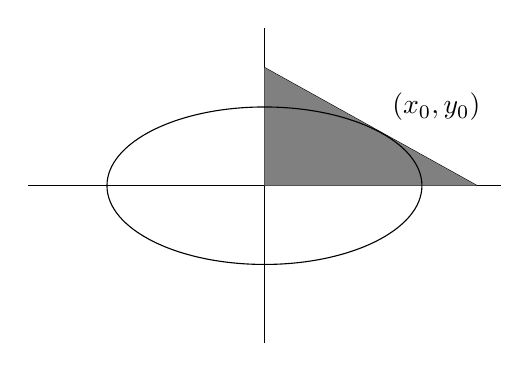
\begin{tikzpicture}
\draw (-3,0) -- (3,0);
\draw (0,-2) -- (0,2);
\draw (0,1.5) -- (2.7,0);
\fill[gray] (0,1.5) -- (2.7,0) -- (0,0) -- cycle;
\draw (0,0) ellipse (2 and 1);
\node [right] at (1.5,1) {$(x_0,y_0)$};
\end{tikzpicture}

$\Delta S = \frac{1}{2} \frac{a^2b^2}{xy}, y=\frac{1}{b} \sqrt{1-\frac{x^2}{a^2}}$

$极值点(\frac{a}{\sqrt{2}},\frac{b}{\sqrt{2}})$

$\\$

T型河道,求船最大能够过的长度

\begin{tikzpicture}
\draw (0,3) -- (1,3);
\draw (1,0) -- (1,3);
\draw (4,0) -- (4,3);
\draw (5,3) -- (4,3);
\draw (0,5) -- (5,5);
\draw[<->] (1,1) -- (4,1);
\node at (2.5,1) {a};
\draw[<->] (0.5,3) -- (0.5,5);
\node at (0.5,4) {b};
\draw (3.5,2) -- (4.5,4);
\node [left] at (4,2) {$\theta$};
\draw (3.75,2.5) arc (240:270:0.5);

\end{tikzpicture}


$l=\frac{a}{sin \theta}+\frac{b}{cos \theta}=a·csc \theta+b·sec \theta$

$l'=a·-ctgx·cscx+b·tgx·secx=a·-\frac{cos\theta}{sin \theta} \frac{1}{sin \theta}+b·\frac{sin \theta}{cos \theta} \frac{1}{cos \theta}$

$tg^3 \theta = \frac{a}{b}$

$\xtx{0} \frac{1}{x^4}[ln(1+sin^{12}x)-6(\sqrt[3]{2-cosx}-1)]$
\end{document}

